% Title: gl2ps_renderer figure
% Creator: GL2PS 1.4.2, (C) 1999-2020 C. Geuzaine
% For: Octave
% CreationDate: Tue Oct 26 12:55:08 2021
\setlength{\unitlength}{1pt}
\begin{picture}(0,0)
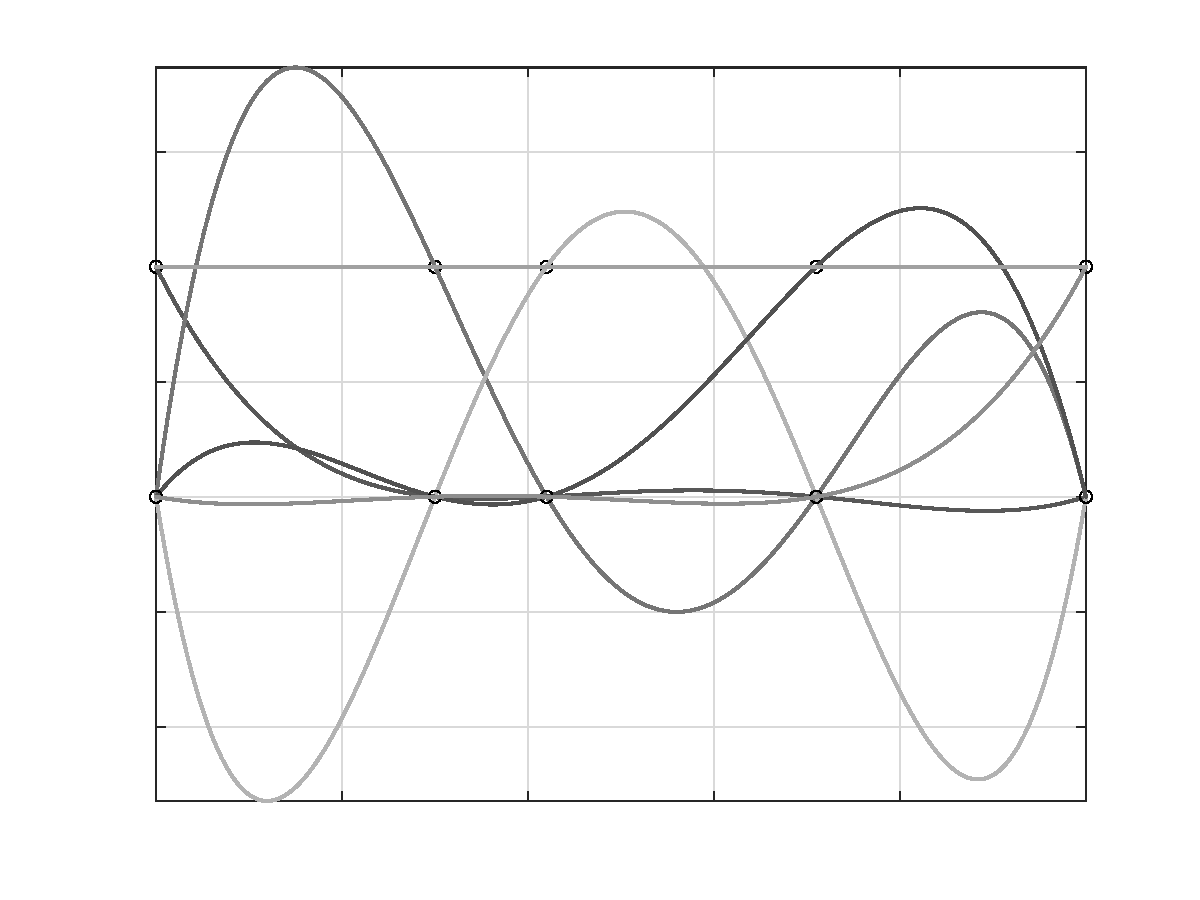
\includegraphics[scale=1]{figures/chap09/OUT/lagrangeBasis04Gray-inc}
\end{picture}%
\begin{picture}(576,432)(0,0)
\fontsize{10}{0}\selectfont\put(74.8799,40.0181){\makebox(0,0)[t]{\textcolor[rgb]{0.15,0.15,0.15}{{0}}}}
\fontsize{10}{0}\selectfont\put(164.16,40.0181){\makebox(0,0)[t]{\textcolor[rgb]{0.15,0.15,0.15}{{0.2}}}}
\fontsize{10}{0}\selectfont\put(253.44,40.0181){\makebox(0,0)[t]{\textcolor[rgb]{0.15,0.15,0.15}{{0.4}}}}
\fontsize{10}{0}\selectfont\put(342.72,40.0181){\makebox(0,0)[t]{\textcolor[rgb]{0.15,0.15,0.15}{{0.6}}}}
\fontsize{10}{0}\selectfont\put(432,40.0181){\makebox(0,0)[t]{\textcolor[rgb]{0.15,0.15,0.15}{{0.8}}}}
\fontsize{10}{0}\selectfont\put(521.28,40.0181){\makebox(0,0)[t]{\textcolor[rgb]{0.15,0.15,0.15}{{1}}}}
\fontsize{10}{0}\selectfont\put(69.8755,83.1758){\makebox(0,0)[r]{\textcolor[rgb]{0.15,0.15,0.15}{{-1}}}}
\fontsize{10}{0}\selectfont\put(69.8755,138.382){\makebox(0,0)[r]{\textcolor[rgb]{0.15,0.15,0.15}{{-0.5}}}}
\fontsize{10}{0}\selectfont\put(69.8755,193.587){\makebox(0,0)[r]{\textcolor[rgb]{0.15,0.15,0.15}{{0}}}}
\fontsize{10}{0}\selectfont\put(69.8755,248.793){\makebox(0,0)[r]{\textcolor[rgb]{0.15,0.15,0.15}{{0.5}}}}
\fontsize{10}{0}\selectfont\put(69.8755,304){\makebox(0,0)[r]{\textcolor[rgb]{0.15,0.15,0.15}{{1}}}}
\fontsize{10}{0}\selectfont\put(69.8755,359.206){\makebox(0,0)[r]{\textcolor[rgb]{0.15,0.15,0.15}{{1.5}}}}
\fontsize{11}{0}\selectfont\put(298.08,27.0181){\makebox(0,0)[t]{\textcolor[rgb]{0.15,0.15,0.15}{{$x$}}}}
\fontsize{11}{0}\selectfont\put(298.08,409.6){\makebox(0,0)[b]{\textcolor[rgb]{0,0,0}{{Lagrange basis functions of degree 4}}}}
\end{picture}
